\documentclass[12pt, specialist, subf, substylefile = spbu.rtx]{disser}
\usepackage[a4paper, includefoot,
            left=3cm, right=1.5cm,
            top=2cm, bottom=2cm,
            headsep=1cm, footskip=1cm]{geometry}
\usepackage[utf8]{inputenc}
\usepackage[T1, T2A]{fontenc}
\usepackage[english, russian]{babel}
\usepackage{moreverb}
\usepackage{array}
\usepackage{hyperref}
\usepackage{amsthm}

\makeatletter
\newcommand{\@chapapp}{\relax}
\makeatother

\usepackage[title,toc,titletoc,header]{appendix}
\setcounter{tocdepth}{2}
\graphicspath{{diploma3_fig/}}
\newtheorem{theorem}{Теорема}
\newtheorem{definition}{Определение}
\newtheorem{algo}{Алгоритм}
\newcommand{\Expect}{\mathsf{E}}
\newcommand{\CVaR}{\mathsf{CVaR}}
\newcommand{\Var}{\mathsf{Var}}
\DeclareGraphicsExtensions{.pdf,.png}
\DeclareMathOperator*{\toplim}{\overline\lim}
\DeclareMathOperator*{\botlim}{\underline\lim}
\DeclareMathOperator*{\tou}{\longrightarrow}
\newcommand{\MDA}{\mathsf{MDA}}
\begin{document}

% Титульный лист


\institution{%
    Санкт-Петербургский государственный университет \\
    Прикладная математика и информатика \\
    Статистическое моделирование
}

\title{Выпускная квалификационная работа}
\topic{\normalfont\scshape %
Доверительное оценивание статистик экстремальных значений}
\author{Старков Артём Константинович}
\group{16.М03-мм}


\sa {М.\,С.~Ермаков}
\sastatus{д.\,ф.-м.\,н., профессор}

\rev {Г.\,Л.~Шевляков}
\revstatus{д.\,ф.-м.\,н., профессор}

\city{Санкт-Петербург}
\date{\number\year}

\maketitle

% titlepage 

\institution{
    Saint Petersburg State University \\
    Applied Mathematics and Computer Science \\
    Statistical Modelling
}
%
\title{Graduation Project}

\topic{\normalfont\scshape 
    Confidence estimation of extreme values statistics}

\author{Starkov Artyom Konstantinovich}

\sa       {M.\,S.~Ermakov}
\sastatus {Professor}

\rev {G.\,L.~Shevlyakov}
\revstatus{Professor}

\city{Saint Petersburg}
\date{\number\year}

\maketitle[en]



\tableofcontents


\intro
%% Введение

События, имеющие малую вероятность, встречаются во многих отраслях человеческой деятельности, таких как строительство, страхование, менеджмент, финансы и др. При этом часто возникают ситуации, когда наблюдения, описывающиеся этими событиями, принимают существенно большие значения, чем остальные наблюдения в выборке. Это порождает задачи оценки тяжести хвоста распределения.

Существует множество работ, вводящих различные характеристики для оценки показателя степени при степенном убывании распределения на хвосте, такие как оценка Хилла~\cite{Hill}, момент-оценки Dekkers ~\cite{dekkers1989}, Pickands estimator~\cite{iii1975} и другие. В статистике экстремальных значений показатель степени убывания хвоста распределения называется параметром формы (shape). Наиболее изученной и широко используемой оценкой этого параметра является оценка Хилла~\cite{Hill}.

Оценка Хилла строится на основе наблюдения редких событий, и в условиях ограниченности размера выборки это особенно подчеркивает необходимость построения доверительного интервала вследствие ее неустойчивости. Построение доверительного интервала имеет малый уровень значимости, и его вычисление может быть достаточно ресурсоемким. В таких случаях могут использоваться различные методы оптимизации для построения доверительных интервалов. Одним из таких методов является метод существенной выборки. Он позволяет уменьшить дисперсию случайной величины при моделировании методом Монте-Карло, путем замены исходной вероятностной меры на смещенное распределение, выделяющее области с более высокой вероятностью для данного конкретного алгоритма.

Данная работа посвящена построению доверительных интервалов для оценки Хилла путем статистического моделирования по методу существенной выборки. Работа разделена на теоретическую и практическую части. В теоретической части будет рассмотрен оцениваемый параметр формы предельного распределения с использованием статистики оценки Хилла; описаны возможности использования метода существенной выборки в задачах оценки малых вероятностей и приведен общий вид вероятностной меры, на основе которой осуществляется эффективное моделирование методом существенной выборки. 

В практической части будут продемонстрированы расчеты, связанные с поиском эффективной меры моделирования, описан алгоритм моделирования случайной величины, распределенной по этой мере. Будут приведены результаты моделирования доверительных интервалов и оценена эффективность примененного метода в сравнении с прямой оценкой.


% Теоретическая часть

\chapter{Теоретическая часть}

\section{Предельные распределения}

В вопросах оценивания вероятностей больших уклонений весьма важную роль играет вопрос о распределении максимумов. Например, пусть дана последовательность независимых одинаково распределенных случайных величин $(X_i)_{i=1}^n$. Будем называть $M_n$ их выборочным максимумом: 
$$
M_1=X_1, \ 
M_n=\max(X_1, ..., X_n).
$$

Одним из результатов изучения распределения $M_n$ является теория предельных распределений. Важный результат этой теории заключен в следующей теореме:
\begin{theorem}[{Фишера-Типпета-Гнеденко~\cite[стр.~121]{Embrechts}}]\label{th:ftg}
Пусть $(X_i)_{i=1}^n$ --- последовательность независимых, одинаково распределенных случайных величин, $M_n$ --- их выборочный максимум $M_n=\max(X_1, ..., X_n).$ Если существуют такие $c_n>0, d_n \in \mathbb{R}$ и некоторая плотность распределения $H$, что выполняется
$$
\frac{(M_n-d_n)}{c_n} \tou^p H,
$$
тогда $H$ принадлежит одному из семейств предельных распределений:

\begin{tabular}{lll}
\text{Фреше:} 
	& $ \Phi_\alpha(x)=e^{-x^{-\alpha}}, $ 
	& $ x>0, \alpha>0; $ \\
\text{Вейбулл:} 
	& $ \Psi_\alpha(x)=e^{-(-x)^\alpha}, $ 
	& $ x \le 0, \alpha>0; $ \\
\text{Гумбель:}
	& $ \Lambda(x)=e^{-e^{-x}}, $ 
	& $ x \in \mathbb{R}. $ \\
\end{tabular}
\end{theorem}

Очевидно, что вид предельного распределения напрямую зависит от распределения случайных величин $X_i$. 
\begin{definition}
Будем говорить, что если некоторая последовательность $(X_i)_{i=1}^n$ с функцией распределения $F(x)$ имеет предельное распределение $H$, то она принадлежит его области максимального притяжения (maximum domain attraction), и записывать:
$$
F \in \MDA(H).
$$
\end{definition}

В данной работе рассматривается предельное распределение Фреше. Оно соответствует семействам распределений Парето, Коши, Булла и др.

Распределение Фреше имеет параметры shape $\alpha>0$, scale $s>0$ и location $m<x$:
$$ F(x)=e^{-(\frac{x-m}{s})^{-\alpha}}, $$
$$ p(x)=\frac{\alpha}{s} \left(\frac{x-m}{s}\right)^{-1-\alpha} e^{-(\frac{x-m}{s})^{-\alpha}}.$$

\begin{theorem}[{\cite[стр.~131]{Embrechts}}]\label{th:freclim}
Функция распределения $F(x)$ принадлежит области максимального притяжения распределения Фреше $F \in \MDA(\Phi_\alpha)$ для $\alpha > 0$, если и только если $\bar{F}(x)=x^{-\alpha}L(x),$ для некоторой медленно меняющейся функции $L$, где $\bar{F}(x)=1-F(x)$ --- распределение хвоста $F(x)$.
\end{theorem}

На основании этого факта Хиллом была получена оценка для $\alpha$, совпадающая с оценкой максимального правдоподобия~\cite{Hill}:
\begin{equation}\label{eq:hillEstLower}
\hat{\alpha}_H=\left(\frac{1}{k} \sum\limits_{i=1}^k \ln X_{i:n}-\ln X_{k:n} \right)^{-1},
\end{equation}
где $k=k(n) \to \infty$. Это оценка <<нижнего>> хвоста (\textit{lower tail estimate}), в той же статье делается оценка и <<верхнего>> хвоста (\textit{upper tail estimate}), то есть для распределения хвоста на интервале $[\beta, 1)$. Она идентична~\eqref{eq:hillEstLower} и делается путем замены $X=Y^{-1}$; соответственно с учетом смены направления упорядочивания вариационного ряда получаем выражение
$$
Y_{i:n}=X_{n-i+1:n},
$$
\begin{equation}\label{eq:hillEst}
\left(\frac{1}{n-m+1} \sum\limits_{i=m}^n \ln X_{i:n}-\ln X_{m:n} \right)^{-1},
\end{equation}
где $m=n-k+1, m=[\beta n]$.

Для многих прикладных задач параметр $\alpha$ имеет большое значение. 
Он используется в качестве индикатора тяжести хвоста распределения. Кроме оценки Хилла, существует большое количество других статистик, оценивающих тяжесть хвоста, например оценка Пиканда~\cite{iii1975}, qq-estimator~\cite{kratz1995}, оценка гармонического момента~\cite{henry2009}, оценка для зависимых гетерогенных даных~\cite{hill2010}, а так же различные вариации на основе оценки~\eqref{eq:hillEstLower} (Resnick 1997~\cite{resnick1998}, Gomes and Martins 2001~\cite{Gomes2001} и др.).

В условиях ограниченности выборки возникает задача определения качества полученной оценки. Так как оценка строится в условиях $k=k(n) \to \infty$, то любая попытка определения качества оценки затруднительна ввиду необходимости получения большого количества реализаций $n \to \infty$ при том, что действительно полезных из них будет относительно немного (в зависимости от параметра $\beta$). В решении этой проблемы в задачах статистического моделирования может помочь асимптотическая эффективность метода существенной выборки.

%% Метод существенной выборки
\section{Метод существенной выборки}

\begin{definition}
Метод существенной выборки (выборка по значимости, importance sampling) -- общая техника оценивания свойств частичных распределений, при которой осуществляется замена вероятностной меры на более соответстующую носителю рассматриваемой статистики.
\end{definition}

Задача для получения доверительных оценок с использованием метода существенной выборки формулируется следующим образом. Пусть $P_0$ -- теоретическое распределение; $\hat{P}_n$ -- эмпирическая функция распределения; $T(P)$ -- некоторый функционал. Вероятность уклонения истинного значения статистики $T(P_0)$ от ее оценки $T(\hat{P}_n)$ не более чем на некоторое значение $b \in R$:
\begin{equation}\label{eq:sv_pt}
\omega=P(T(\hat{P}_n)-T(P_0) > b).
\end{equation}

Для получения оценки этой вероятности выбирается абсолютно непрерывная к $P_0$ вероятностная мера $Q$; по ней моделируются $K$ независимых выборок:
$$
Y_1^{(k)}, Y_2^{(k)}, ... , Y_n^{(k)}, 1 \le k \le K.
$$

Тогда оценка вероятности~\eqref{eq:sv_pt}:
\begin{equation}\label{eq:sv_sd}
\hat{\omega}_n=\frac{1}{K} \sum\limits_{k=1}^{K}
\chi \big(T(\hat{Q}^{(k)}_n)-T(P_0) > b_n\big)
\prod\limits_{j=1}^{n} q_n^{-1}(Y_j^{(k)}),
\end{equation}
где $\hat{Q}^{(k)}_n$ -- эмпирическое распределение выборки $Y^{(k)}_j$, $q_n=\frac{dQ_n}{dP_0}$.

Дисперсия оценки~\eqref{eq:sv_sd} имеет вид
\begin{equation}\label{eq:est_disp}
V(Q_n)=\Var[\hat\omega_n]=U_n-\omega_n^2,
\end{equation}
где $\omega_n$ -- математическое ожидание~\eqref{eq:sv_sd},
$$
U_n=\Expect_{Q_n} 
\left[   
\chi \big(T(\hat{Q}^{(1)}_n)-T(P) > b_n\big)
\prod\limits_{j=1}^{n} q_n^{-2}(Y_j^{(1)})
\right],
$$

Так как $U_n$ и $\omega_n$ -- малые величины, то естественно рассматривать асимптотическую эффективность процедуры существенной выборки. 

\begin{definition}
Процедура называется асимптотически эффективной (в смысле логарифмической асимптотики), если 
$$
\overline{\lim\limits_{n \to \infty}} \frac{\log U_n}{\log \omega_n^2} = 1.
$$
\end{definition}

Основной трудностью при использовании метода существенной выборки является выбор меры $Q_n$, при котором процедура асимптотически эффективна или близка к такой.

Предпосылкой для решения задачи о выборе меры $Q_n$ стала работа математика И. Н. Санова~\cite{Sanov1957}. Им была исследована задача вычисления вероятности 
\begin{equation}\label{eq:sv_san}
P(\hat{P}_n \in \Omega),
\end{equation}
где $\hat{P}_n$ -- эмпирическая функция распределения, построенная по выборке $X_i \sim P_0, 1 \le i \le n$; $\Omega$ принадлежит пространству мер. Он исследовал асимптотическое поведение вероятности~\eqref{eq:sv_san} и получил следующие результаты:
\begin{equation}\label{eq:sv_san2}
\begin{tabular}{l}
$\toplim\limits_{n \to \infty} \frac{1}{n} \ln P(\hat{P}_n \in \Omega) \le -\inf\limits_{Q\in \mathfrak{int}(\Omega)} K(Q, P_0),$
\\
$\botlim\limits_{n \to \infty} \frac{1}{n} \ln P(\hat{P}_n \in \Omega) \ge -\inf\limits_{Q\in \mathfrak{cl}(\Omega)} K(Q, P_0),$
\end{tabular}
\end{equation}
где $\mathfrak{int}(\Omega)$ и $\mathfrak{cl}(\Omega)$ -- соответственно замыкание и внутренность $\Omega$ в специальной топологии со слабой сходимостью, 
\begin{equation}\label{eq:sv_k}
K(Q, P_0)=
\begin{cases}
\int \ln \frac{dQ}{dP_0}dQ, 
	&\text{если $Q \ll P_0$;}\\
\infty,	
	&\text{иначе.}
\end{cases}
\end{equation}

На основе этих результатов в дальнейшем была развита теория вероятности больших уклонений, окончательно формализованная С. Р. Варадханом. В рамках этой теории неравенства типа~\eqref{eq:sv_san2} стали называться принципом больших уклонений, а функционалы типа~\eqref{eq:sv_k}
-- функционалами действия. Они являются в некотором смысле мерой близости распределений $Q$ и $P_0$, схожей с расстоянием Кульбака-Лейблера.

Задача~\eqref{eq:sv_pt} может быть рассмотрена при разных ограничениях, наложенных на $b$. Для случая больших уклонений нахождение эффективной меры $Q$ в общем случае является неразрешимой задачей. В зоне умеренных уклонений и действия ЦПТ для задачи в виде
\begin{equation}\label{eq:sv_ptum}
P(T(\hat{P}_n)-T(P_0) > b_n), 
\end{equation}
где $nb_n^2 \to \infty, b_n \to 0, b_n > 0$, действует нормальная асимптотика, в смысле логарифма аппроксимации. Здесь задача нахождения $Q$ разрешима для очень широкого класса функционалов $T$.

М. Джонсом была построена асимптотически эффективная процедура метода существенной выборки в зоне нормальной аппроксимации. На зону умеренных уклонений его результаты были перенесены М. С. Ермаковым в статье~\cite{Ermakov}. В статье рассматривается задача~\eqref{eq:sv_ptum} в случае, когда статистика $T(\hat{P}_n)$ имеет функцию влияния $g$ и верны предположения, рассматриваемые ниже.

Введем следующие множества: 
\begin{enumerate}
\item множество функций $\Phi$ такое, что для любой $f \in \Phi$  $\Expect f(x)=0 $ и
$$
\lim\limits_{n \to \infty} \frac{1}{nb_n^2} \log \big(nP_0(|f(X)|>nb_n)\big)=-\infty;
$$

\item множество $\Lambda_\Phi$ всех мер $Q \in \Lambda$ таких, что для любой $f \in \Phi$
$
\int\limits_{\Omega} |f| dQ < \infty;
$

\item множество $\Lambda_{0\Phi}$ всех зарядов $G=P-R; P, R \in \Lambda$.

\end{enumerate}

Тогда предположим, что $g \in \Phi$ и существует полунорма $N \in \Lambda_{0\Phi}$, такая, что для любого $Q \in \Lambda_\Phi$
$$
|T(Q)-T(P_0)-\int\limits_{\Omega}g dQ| \le 
\omega\left(N(Q-P_0),\ \int\limits_{\Omega}g dQ,\ T(Q)-T(P_0) \right)
$$
с функцией $\omega\colon \mathbb{R}^3 \to \mathbb{R}_+$, такой, что
$$
\lim\limits_{t_1, t_2, t_3 \to 0} \frac{\omega(t_1, t_2, t_3)}{t_1+ t_2+t_3} = 0.
$$

М. С. Ермаковым была доказана следующая теорема.
\begin{theorem}[{\cite{Ermakov}}]\label{th:erm}
В предположениях, изложенных выше, рассмотрим процедуру существенной выборки, основанную на вероятностной мере $Q_n$ с плотностью 
$$
q_{1n}(x)=\lambda_n+b_nh(x)\chi\left(h(x)>-\frac{\delta}{b_n}\right)
$$
или
$$
q_{2n}(x)=c_ne^{b_nh(x)} \chi\left(h(x)<\frac{\delta}{b_n}\right),
$$
где $\lambda_n, c_n$ -- константы нормализации, $\delta \in [0, 1]$ и $\Expect h(x)=0, \Expect|h(x)|<\infty, \Expect h^2(x)< \infty$. Тогда процедура существенной выборки асимптотически эффективна, если $h=\frac{g}{\sigma^2_g}$

\end{theorem}


%% Постановка задачи
\section{Постановка задачи}

Пусть $(X_i)_{i=1}^n$ --- независимые случайные величины с функцией распределения $F \in \MDA(\Phi_\alpha)$. Упорядочим выборку по возрастанию, получим вариационный ряд:
$$
X_{1:n} \le X_{2:n} \le ... \le X_{n:n}.
$$

Распределение хвоста $\bar{F}(x)=1-F(x)$ принадлежит семейству предельных распределений Фреше $\Phi_\alpha$, в котором неопределенным остается параметр формы (shape) $\alpha$. Имеем для него оценку Хилла:
\begin{equation}\label{eq:hill_est}
\hat{\alpha}_H=
\left(\frac{1}{n-m+1} \sum\limits_{i=m}^n \ln X_{i:n}-\ln X_{m:n} \right)^{-1},
\end{equation}
где $m=[\beta n]$.

Рассмотрим задачу оценки вероятности уклонения оцененного значения от истинного, представленной в формуле~\eqref{eq:sv_pt}, где в качестве функционала $T(F)$ будет выступать оценка $\hat{\alpha}_H$. Так как сама оценка строится в условиях $m=m(n) \to \infty$, то обычные оценки становятся неэффективными. Для решения данной проблемы будет использована асимптотическая эффективность метода существенной выборки.

По теореме \ref{th:erm} будем использовать вероятностную меру $Q_n$ вида
\begin{equation}\label{eq:g_common}
g(x)=p(x)(1+b_nh(x)),
\end{equation}
где $h(x)$ --- функция влияния оцениваемого функционала, $b_n$ -- константа для определения ширины доверительного интервала, 

\begin{equation}\label{eq:bn}
b_n = \pm\frac{N_{(0,1)}^{-1}(\gamma)}{\sqrt{n}\sigma},
\end{equation}

\begin{equation}\label{eq:asymdisp}
\sigma^2(F)= \int_{-\infty}^\infty \int_{-\infty}^\infty J(F(x)) J(F(y))\big( F(x \wedge y)-F(x)F(y)\big)
\end{equation}
--- асимптотическая дисперсия функционала $T(F)$.

Целью данной работы является построение доверительного интервала вероятности вида~\eqref{eq:sv_pt} для функционала оценки Хилла. Для ее достижения необходимо:

\begin{enumerate}

\item определить внешний вид функционала $T(P)$, его функцию влияния и дисперсию~\eqref{eq:asymdisp};

\item определить и промоделировать вспомогательное распределение $Q_n$~\eqref{eq:g_common};

\item на основе модельных данных построить доверительный интервал для вероятности~\eqref{eq:sv_sd};

\item оценить вычислительную эффективность данной оценки по сравнению с прямым методом.

\end{enumerate}

%% Моделирование
\chapter{Моделирование}

\section{Оцениваемый функционал}

В данной работе рассматривается оценка Хилла верхнего хвоста предельного распределения~\eqref{eq:hill_est}. Используя теорему~\ref{th:freclim}, и при допущении $L(x)=const$ сделаем замену:
\begin{equation}\label{eq:rep_xy}
F(x)=1-Cx^{-\alpha}|_{\ln x=y}=1-Ce^{-\alpha y}=exp(y; \alpha).
\end{equation}

Исходя из этого, получаем, что распределение исходной случайной величины становится экспоненциальным с параметром $\alpha$. Кроме этого, для удобства будем оценивать не $\hat{\alpha}_H$, а $\hat{\alpha}_H^{-1}$. С учетом данных замечаний, функционал оценки принимает следующий вид:
\begin{equation}\label{eq:t_f_y}
T(F_y)=\hat{\alpha}_H^{-1}=\frac{1}{n-m+1} \sum\limits_{i=m}^n Y_{i:n}- Y_{m:n}
\end{equation}


Общий вид таких функционалов для L-оценок предложен в книге Serfling~\cite[стр.~263]{Serfling}:
\begin{equation}\label{eq:t_f_common}
T(F)=\int\limits_0^1 F^{-1}(t)J(t)dt + \sum\limits_{j=1}^l a_jF^{-1}(p_j),
\end{equation}
где $J(t)$ --- некоторая интегрируемая весовая функция, $p_j$ --- уровни квантилей $F^{-1}(p_j),$ $a_j$ -- соответствующие им веса. 

Там же предложен общий вид функции влияния:
$$
IC(x; T, F)=-\int\limits_{-\infty}^\infty [\chi(x \le y) - F(y)]J(F(y))dy+ \sum\limits_{j=1}^l a_j\frac{p_j-\chi(x \le F^{-1}(p_j))}{f(F^{-1}(p_j))}.
$$

Перепишем~\eqref{eq:t_f_y} с учетом формы~\eqref{eq:t_f_common}:
$$
T(F_y)=\frac{1}{n-m+1} \sum\limits_{i=m}^n Y_{i:n}-Y_{m:n}=
\frac{1}{n-m+1} \sum\limits_{i=m}^n F_y^{-1}(\frac{i}{n})-F_Y^{-1}(\beta)=
$$
\begin{equation}\label{eq:t_hill_res}
=\frac{1}{1-\beta} \int\limits_\beta^1 F_y^{-1}(t) dt-F_y^{-1}(\beta),
\end{equation}
\begin{equation}\label{eq:jt}
J(t)=\frac{\chi(t>\beta)}{1-\beta}.
\end{equation}

Соответственно функция влияния принимает вид:
$$
h(x)=IC(x; T, F_y)=\frac{1}{\beta-1}\int\limits_{F_y^{-1}(\beta)}^\infty 
(\chi(x \le t) - F_y(t))dt- \frac{\beta-\chi(x \le F_y^{-1}(\beta))}{f_y(F_y^{-1}(\beta))};
$$
Обозначив $F_y^{-1}(\beta)=x_1$, получаем:
\begin{equation}\label{eq:h_cases}
h(x)=
\begin{cases}
\frac{1}{\beta-1}\int\limits_{x_1}^\infty (1-F_y(t))dt-\frac{\beta-1}{f_y(x_1)}, 
	&\text{если $x \le x_1$;} \\
\frac{1}{1-\beta}\int\limits_{x_1}^x F_y(t)dt+\frac{1}{\beta-1}\int\limits_x^\infty(1-F_y(t))dt-\frac{\beta}{f_y(x_1)} , 
	&\text{иначе.}
\end{cases}
\end{equation}

Используя~\eqref{eq:rep_xy}, подставим функцию распределения как экспоненциальную с параметром $\alpha$:

\begin{equation*}
h(x)=
\begin{cases}
\frac{1}{\alpha(\beta-1)}\big(e^{-\alpha x_1} +\beta-1\big),
	&\text{если $x \le x_1$;}\\
\frac{1}{\alpha(1-\beta)}\big(\alpha(x-x_1)- e^{-\alpha x_1}-\beta\big),
	&\text{иначе.}
\end{cases}
\end{equation*}

Заметим, что 
$$
e^{-\alpha x_1}=
e^{-\alpha F^{-1}(\beta)}=
e^{-\alpha \left(-\frac{1}{\alpha}\ln(1-\beta)\right)}=
e^{\ln(1-\beta)}=
1-\beta.
$$
Также обозначим $x_2=h^{-1}(0)=\frac{1}{\alpha}+x_1$. С учетом этого получаем итоговую функцию для $h(x)$:
\begin{equation*}
h(x)=\frac{x-x_2}{1-\beta}\chi(x>x_1).
\end{equation*}

Функция распределения~\eqref{eq:g_common} принимает вид:
\begin{equation}\label{eq:g_final}
g(x) = p(x)(1+b_nh(x))=\alpha e^{-\alpha x}\left(1 + b_n\frac{x-x_2}{1-\beta}\chi(x > x_1) \right).
\end{equation}

Для моделирования требуется знать интеграл функции~\eqref{eq:g_final} на произвольном промежтке $[a, b] \in [x_1, \infty)$:

$$
\int \limits_a^b g(x)dx=
\int \limits_a^b \alpha e^{-\alpha x}(1+b_n\frac{x-x_2}{1-\beta})dx = 
$$
\begin{equation}\label{eq:gint}
=(e^{-\alpha a}-e^{-\alpha b})(1-\frac{b_n x_2}{1-\beta})-
\frac{b_n}{\alpha(1-\beta)}\left(e^{-\alpha b}(\alpha b+1)-e^{-\alpha a}(\alpha a+1)\right).
\end{equation}

Вывод дисперсии функционала оценки осуществляется по формуле~\eqref{eq:asymdisp}. Он приведен в приложении~\ref{sec:app_disp}. Итоговая дисперсия функционала оценки~\eqref{eq:sigma_res}:
$$
\sigma^2(F)= \frac{\beta + 1}{\alpha^2(1-\beta)}
$$

При использовании $b_n < 0$ изменяется функция $g(x)$, потому для нее строится распределение, отличное от случая $b_n > 0$.

% b_n > 0

\section{Случай $b_n > 0$}

Решается задача вычисления оценки~\eqref{eq:sv_sd} в исходой форме:

\begin{equation}\label{eq:est_plus}
\hat{\omega}_n=\frac{1}{k} \sum\limits_{i=1}^{k}
\chi \big(T(\hat{Q}^{(i)}_n)-T(P_0) > b_n\big)
\prod\limits_{j=1}^{n} 
\frac{1}{1+b_nh(Y_j^{(i)})},
\end{equation}

Разобьем область моделирования на 3 части: 
$$0 \le A < x_1 \le B \le x_2 \le C < \infty.$$

В каждой области функция имеет свои особенности. Внешний вид плотности распределения показан на рисунке~\ref{ris:plot1}. 

\begin{figure}[h]
\center{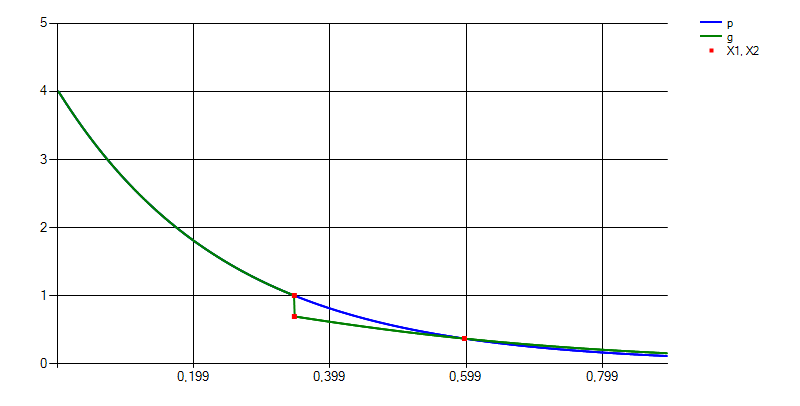
\includegraphics[width=1\linewidth]{plot1}}
\caption{Распределение $g(x), p(x)$ и точки $x_1, x_2$}
\label{ris:plot1}
\end{figure}


% A 1

\subsection{Область $A=[0, x_1)$}

Область $A$ не отличается от исходного показательного распределения. Моделирование проводится методом обратной функции. Интеграл $\int_A g(x) dx = \beta$.

% B 1

\subsection{Область $B=[x_1, x_2)$}

Моделирование проходит по алгоритму метода мажорант~\cite{MonErm}:

\begin{algo}[Метод мажорант]\label{algo:mag}
Пусть 
$$
D_S=\frac{\int_S p(x) dx}{\int_S q(x) dx},
$$
где $q(x)$ --- моделируемая плотность, $p(x)$ --- некоторая другая плотность, такая, что $\forall x \in S \ p(x) \ge q(x)$. Тогда:
\begin{enumerate}
\item получим реализацию $\xi \sim \frac{p(X)}{|D|}$;
\item получим реализацию $\eta_{s+1} \sim U(0, p(\xi))$;
\item если $\eta_{s+1} > q(\xi)$, переходим к пункту 1; иначе $\xi$ --- искомая случайная величина, $\xi \sim q(x)$.
\end{enumerate}

Эффективность метода равна $\frac{1}{|D_S|}$.
\end{algo}

В данной области искомая плотность $g(x)$ мажорируется экспоненциальной плотностью распределения $p(x)$. Эффективность метода:
$$
\frac{1}{|D_S|}=1-\frac{b_n}{\alpha(e-1)(1-\beta)}.
$$

% C 1

\subsection{Область $C=[x_2, \infty)$}

В области $C$ используем метод композиции~\cite{MonErm}. 

\begin{algo}[Метод композиции]\label{alg:comp}
Пусть искомая плотность $g(x)$ представлена суммой плотностей $p_i(x)$ с некоторыми неотрицательными весами $a_i$:
\begin{equation}\label{eq:comp_common}
g(x)=\sum\limits_{i=1}^M a_ip_i(x).
\end{equation}

Тогда метод выражается следующим алгоритмом:
\begin{enumerate}
\item получаем реализацию $\xi \sim U(0, \sum_i a_i)$;
\item выбираем индекс $s=\arg\max(a_i:a_i<\xi);$
\item искомая случайная величина --- $\eta \sim p_s(x)$.
\end{enumerate}
\end{algo}

Для использования метода плотность $g(x)$ должна быть представлена в виде суммы плотностей с неотрицательными коэффициентами. Представим функцию в виде:
$$
g(x)=p(x)(1+b_nh(x))=\alpha e^{-\alpha x} + \frac{b_n(x-x_2)}{1-\beta}\alpha e^{-\alpha x}=p(x)+p_1(x).
$$

Заменим во второй части $y=x-x_2$:
$$
p_1(y)=\frac{b_ny}{1-\beta} \alpha e^{-\alpha (y+x_2)}=
\frac{b_n}{\alpha(1-\beta)} \alpha^2 ye^{-\alpha y}e^{-\alpha x_2}=
\frac{b_n}{\alpha e} \alpha^2 ye^{-\alpha y}.
$$

Теперь $p_1(y)$ выражается гамма-распределением с параметрами $shape=2, scale=\frac{1}{\alpha}$. Получаем форму~\eqref{eq:comp_common} с весами $a_1=1, a_2=\frac{b_n}{\alpha e}$ и распределениями 

$$
p_0(x)=p(x)=exp(x, \alpha),
$$ 
$$
p_1(x)=\gamma(x, 2, \frac{1}{\alpha}).
$$

Так как на веса накладывается ограничение неотрицательности, данный метод не может быть применен к области $B$, так как в ней $x < x_2$, и коэффициент $a_2$ при плотности $p_1(x)$ становится меньше нуля.

% sum

\subsection{Общее распределение $g(x), b_n > 0$}

Моделирование проводится при помощи алгоритма~\ref{alg:comp}. В качестве весов берутся интегралы плотности $g(x)$ по соответствующим областям. Пример результата моделирования распределения в виде гистограммы с наложенными функциями $g(x), p(x)$ представлен на рисунке~\ref{ris:hist1}. 

\begin{figure}[h]
\center{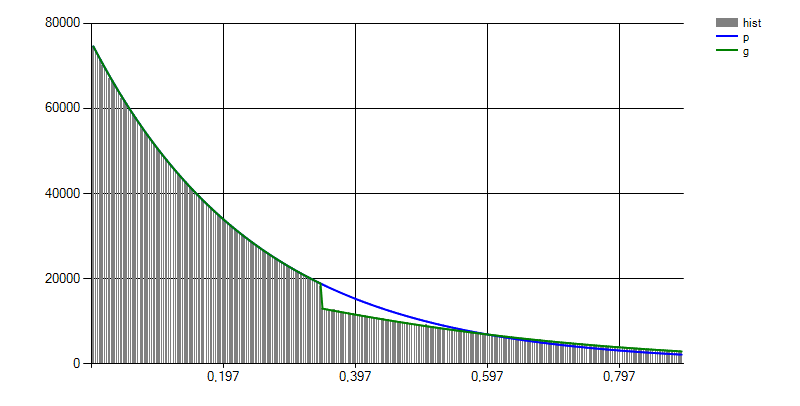
\includegraphics[width=1\linewidth]{hist1}}
\caption{Распределение $g(x), p(x)$}
\label{ris:hist1}
\end{figure}

% b_n < 0

\section{Случай $b_n < 0$}

Для данного случая изменен вид функции $g(x) = p(x)(1-b_n h(x))$, также 
в задаче поиска оценки~\eqref{eq:sv_sd} изменяется индикатор:

\begin{equation}\label{eq:est_minus}
\hat{\omega}_n=\frac{1}{k} \sum\limits_{i=1}^{k}
\chi \big(T(\hat{Q}^{(i)}_n)-T(P_0) < -b_n\big)
\prod\limits_{j=1}^{n} 
\frac{1}{1-b_nh(Y_j^{(i)})},
\end{equation}


Как и в предыдущем разделе, разобьем область моделирования на 3 части. Интегралы соответствующих зон получаются из формул для случая $b_n>0$ при замене знака при $b_n$ на противоположный. Внешний вид плотности распределения показан на рисунке~\ref{ris:plot2}. 

\begin{figure}[h]
\center{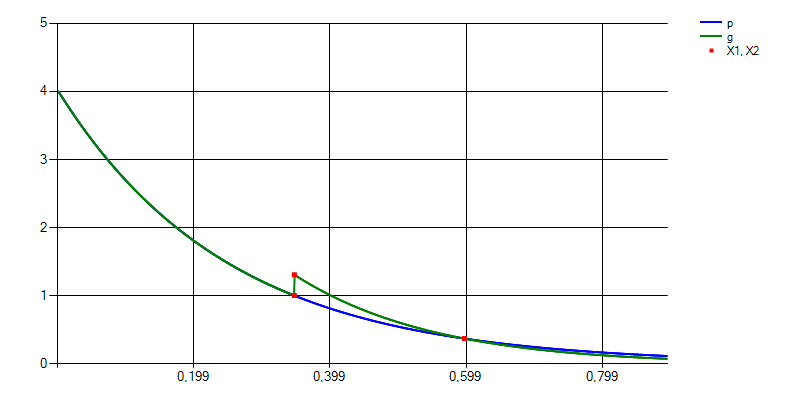
\includegraphics[width=1\linewidth]{plot2}}
\caption{Распределение $g(x), p(x)$ и точки $x_1, x_2$}
\label{ris:plot2}
\end{figure}

% A 2

\subsection{Область $A=[0, x_1)$}

Также, как и в первой части, область $A$ не отличается от исходного показательного распределения. Моделирование проводится методом обратной функции.

% B 2

\subsection{Область $B=[x_1, x_2)$}

Необходимо сгенерировать случайную величину с плотностью
$$
g(x) = p(x)(1-b_n h(x)) = \alpha e^{-\alpha x}(1-b_n \frac{x-x_2}{1-\beta})=
$$
\begin{equation}\label{eq:b2_g}
=\alpha e^{-\alpha x}(1+b_n \frac{x_2-x}{1-\beta})
\end{equation}

Будем проводить моделирование при помощи алгоритма~\ref{algo:mag}. Заметим, что $x_1 \le x \le x_2$, а значит $0 \le x_2-x \le x_2-x_1$.
Так как $(1+b_n \frac{x_2-x}{1-\beta})$ линейная убывающая функция, можем рассмотреть ее максимум на интересующем нас промежутке. Он достигается на $\min x = x_1$. Тогда мажорирующая функция имеет вид
$$
q(x)=\alpha e^{-\alpha x}(1+b_n \frac{x_2-x_1}{1-\beta}).
$$
$$
\int_B q(x)=\frac{e-1}{e}(1-\beta+\frac{b_n}{\alpha}),
$$
Эффективость метода:
$$
\frac{1}{|D_S|}=\frac{1-\beta+\frac{b_n}{\alpha(e-1)}}{1-\beta+\frac{b_n}{\alpha}}.
$$


% C 2

\subsection{Область $C=[x_2, \infty)$}

В области $C$ также используем метод мажорант~\ref{algo:mag}. В данной области $g(x)$ успешно мажорируется функцией $p(x)$. Эффективность метода:
$$
\frac{1}{|D_S|}=\frac{1-\beta+\frac{b_n}{\alpha}}{1-\beta}=1+\frac{b_n}{\alpha(1-\beta)}.
$$


% sum 2

\subsection{Общее распределение $g(x), b_n < 0$}

Моделирование проводится при помощи алгоритма~\ref{alg:comp}. В качестве весов берутся площади плотности $g(x)$ в соответствующих областях. Результат моделирования распределения в виде гистограммы с наложенными функциями $g(x), p(x)$ представлен на рисунке~\ref{ris:hist2}. 

\begin{figure}[h]
\center{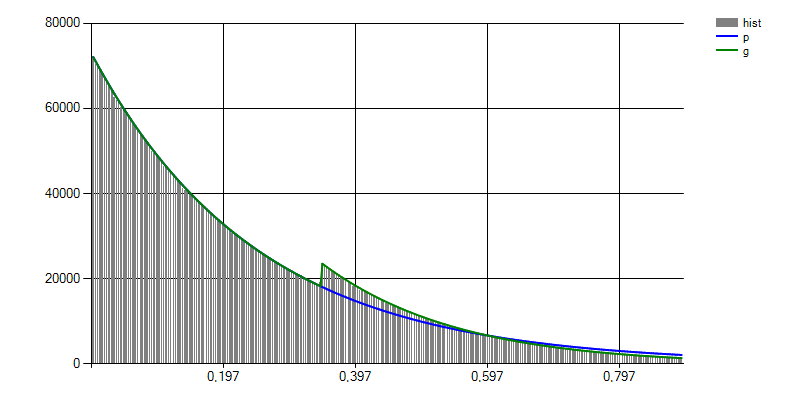
\includegraphics[width=1\linewidth]{hist2}}
\caption{Распределение $g(x), p(x)$}
\label{ris:hist2}
\end{figure}

%
% Построение доверительного интервала
%

\section{Построение доверительного интервала}

При построении доверительного интервала используется соответствующая формула оценки вероятности~\eqref{eq:est_plus} или~\eqref{eq:est_minus}. Дисперсия оценки вычисляется при помощи формулы~\eqref{eq:est_disp}.

Доверительный интервал для оценки значения рассматриваемого функционала c уровнем доверия $\bar{\omega}(\gamma)$ имеет следующий вид: 

\begin{equation}\label{eq:inter_a}
\bar{\alpha}^{-1} = \hat{\alpha}^{-1}_H \pm b_n(\gamma),
\end{equation}

\begin{equation}\label{eq:inter_w}
\bar{\omega}(\gamma) = \hat{\omega}_n(\gamma) \pm \sigma(\hat{\omega}_n(\gamma)).
\end{equation}

Для оценки полученных результатов необходимо получить некоторую оценку, которую можно было бы принять за эталонную. Для этого используется подсчет статистики~\eqref{eq:est_plus} в следующем виде:

\begin{equation}\label{eq:est_direct}
\hat{\omega}_D=\frac{1}{k} \sum\limits_{i=1}^{k}
\chi \big(T(\hat{Q}^{(i)})-T(P_0) > b_n\big),
\end{equation}
где $T(\hat{Q}^{(i)})$ строится по формуле~\eqref{eq:t_f_y} с $Y_i \sim exp(x; \alpha)$. Дисперсия оценки:

$$
D \hat{\omega}_D = \sqrt{\frac{\hat{\omega}_D(1-\hat{\omega}_D)}{k}}.
$$

Оценка~\eqref{eq:est_direct} является прямой оценкой для исходного функционала.


% Результаты
\section{Результаты}

%
% Программа
%

Для генерации случайных величин с требуемой вероятностной мерой, и построения на их основе доверительных интервалов, была написана программа, включающая в себя расчетный модуль и простой пользовательский интерфейс.

Изначально прототип вычислительного модуля разрабатывался в среде разработки R Studio с использованием интерпретируемого языка R. Ввиду неэффективности работы языка R при необходимости большого количества вычислений было принято решение о переносе разрабатываемого вычислительного модуля на платформу .NET, и создание приложения для взаимодействия с ним. Это позволило на 3-4 порядка увеличить скорость проведения вычислений.

Расчетный модуль для генерации распределения и построения доверительных итервалов реализован на языке C\#, платформа .NET 4.0. Для генерации сложных распределений (например, гамма-распределения), используется библиотека Accord.NET. Пользовательский интерфейс программы реализован на базе набора библиотек WinForms в составе платформы .NET. Программа позволяет строить графики зависимости $\gamma$ от $\hat{\omega}_n$ и гистограммы распределения $g(x)$ для случаев $b_n > 0 $ и $b_n < 0$. Поддержана возможность получения графиков для прямой оценки и оценки при помощи метода существенной выборки.

В качестве демонстрации результатов моделирования представлены примеры построения доверительных интервалов для случаев $b_n > 0$ и $b_n < 0$ (рисунок~\ref{ris:imp}, таблица~\ref{table:imp}). Выбор $\beta$ делается исходя из стандартной практики в данной области, ее значение выбирают в зависимости от объема выборки в диапазоне от $0.8$ до $0.9$.

\begin{figure}[h]
\center{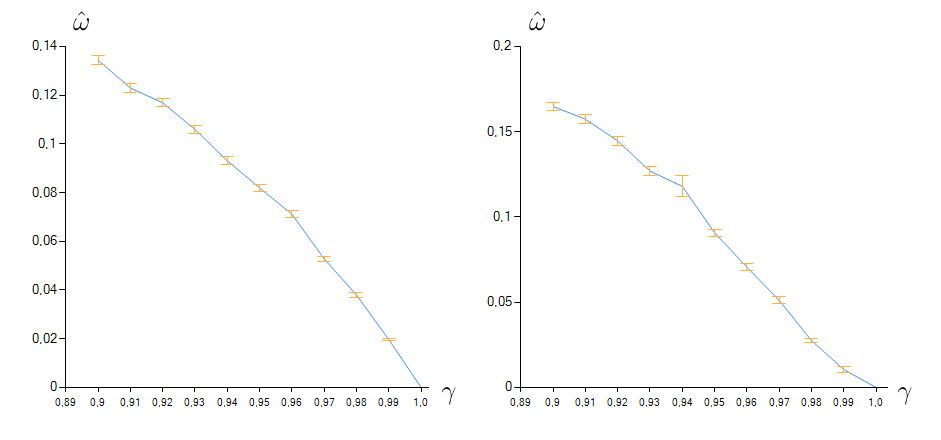
\includegraphics[width=1\linewidth]{imp}}
\caption{Результаты моделирования вероятности уклонения для $k=10000, n=1000, \alpha=2, \eta=0.85; b_n > 0 $ (слева) и $b_n < 0$ (справа)}
\label{ris:imp}
\end{figure}

\begin{table}[ht]
\caption{Результаты моделирования вероятности уклонения для $k=10000, n=1000, \alpha=2, \eta=0.85$} 
\label{table:imp}
\centering
\begin{tabular}{c|cc|cc}
  \hline
$\gamma$ & $\hat{\omega}, b_n > 0$ & $\sigma$ & $\hat{\omega}, b_n < 0$ & $\sigma$ \\ 
  \hline
0.90 & 0.13434 & 0.00194 & 0.16471 & 0.00250 \\ 
0.91 & 0.12288 & 0.00186 & 0.15738 & 0.00266 \\ 
0.92 & 0.11689 & 0.00178 & 0.14455 & 0.00280 \\ 
0.93 & 0.10589 & 0.00170 & 0.12688 & 0.00262 \\ 
0.94 & 0.09306 & 0.00156 & 0.11794 & 0.00605 \\ 
0.95 & 0.08190 & 0.00144 & 0.09071 & 0.00204 \\ 
0.96 & 0.07113 & 0.00142 & 0.07052 & 0.00196 \\ 
0.97 & 0.05274 & 0.00115 & 0.05106 & 0.00211 \\ 
0.98 & 0.03797 & 0.00092 & 0.02747 & 0.00110 \\ 
0.99 & 0.01966 & 0.00059 & 0.01049 & 0.00186 \\ 
1.00 & 0.00000 & 0.00000 & 0.00000 & 0.00000 \\  
   \hline
\end{tabular}
\end{table}

По таблице~\ref{table:imp} можно построить доверительные интервалы по формулам~\eqref{eq:inter_a} и~\eqref{eq:inter_w}. Здесь $\sigma=\sigma(\hat{\omega}_n(\gamma))$, $\hat{\omega}=\hat{\omega}_n(\gamma)$. Значение $\hat{\alpha}_H^{-1}$ оценивается отдельно для произвольной выборки, $b_n(\gamma)$ рассчитывается по формуле~\eqref{eq:bn}.

При построении доверительного интервала фиксируется $\alpha$, затем последовательно выбирается квантиль $\gamma$ из заданного интервала с указанным шагом. Для построения по формуле~\eqref{eq:bn} вычисляется $b_n$, затем моделируется $k$ выборок $Y^{(i)} \sim g(x)$ размера $n$. В качестве $T(\hat{Q}^{(i)}_n)$ берется оценка функционала~\eqref{eq:t_f_y} по выборке $Y^{(i)}$, $T(P_0)=\alpha^{-1}$. Оценивание производится отдельно для случая $b_n > 0$ и $b_n < 0$, так как распределение для метода существенной выборки у них различно.


% Сравнение

Сравнение результатов проводилось для метода существенной выборки и для прямой оценки~\eqref{eq:est_direct}. Сравнивались отклонения для оцененных значений вероятностей $\hat{\omega}$. Сгенерированы оценки с параметрами $\alpha = \{1,2,3,5,10\}; \beta=\{0.80..0.95\}$ с шагом по $0.5; \gamma=\{0.8..0.98\}$ с шагом по 0.2. Доверительные интервалы строились на 1000 выборках по 1000 элементов. В таблице~\ref{table:cmp} представлены полученные среднеквадратичные отклонения в зависимости от перечисленных параметров, с усреднением по параметру~$\gamma$.

% Заключение

\conclusion

В работе исследована задача построения доверительного интервала для вероятности уклонения параметра формы (\textit{shape}), полученного при помощи оценки Хилла. Задача решалась на основе асимптотической эффективной процедуры существенной выборки для $b_n>0$ и $b_n<0$.

Найден явный вид асимптотически эффективной меры моделирования в методе существенной выборки для этой задачи. Предложен алгоритм моделирования случайных величин, соответстующих данной вероятностной мере. Осуществлено моделирование методом существенной выборки. Представлены примеры построения доверительных интервалов, получены результаты сравнения дисперсий данного метода и прямой оценки. 

Представляет интерес провести моделирование доверительных интервалов для других офенок параметра формы shape и таким образом осуществить сравнение качества этих оценок.

\bibliographystyle{gost2008}
\bibliography{diploma3}


\newpage
\appendix
\chapter{Дополнительные расчеты}\label{sec:app_disp}

\section{Дисперсия оценки}

По~\eqref{eq:asymdisp} имеем:

$$
\sigma^2(F)= \int_{-\infty}^\infty \int_{-\infty}^\infty J(F(x)) J(F(y))\big( F(x \wedge y)-F(x)F(y)\big).
$$

В~\eqref{eq:jt} была выражена функция $J(t)$:
$$
J(t)=\frac{\gamma(t>\beta)}{1-\beta},
$$
$$
J(F(t))=\frac{\gamma(F(t)>\beta)}{1-\beta}.
$$

Зафиксируем $y$ и частично выразим~\eqref{eq:asymdisp}:
$$
\int_{-\infty}^\infty \big( F(\min(x, y))-F(x)F(y)\big)dx = 
$$
$$
=\int_{-\infty}^y F(x)dx + \int_y^\infty F(y)dx - 
\int_{-\infty}^\infty F(y)F(x)dx =
$$
$$
=\int_{-\infty}^y F(x)dx + \int_y^\infty F(y)dx - 
\int_{-\infty}^y F(y)F(x)dx -
\int_y^\infty F(y)F(x)dx =
$$
$$
=\int_{-\infty}^y F(x)dx + F(y) \left(
\int_y^\infty dx - 
\int_{-\infty}^y F(x)dx -
\int_y^\infty F(x)dx
\right)=
$$
$$
=
\int_{-\infty}^y F(x)dx + F(y) \left(
\int_y^\infty (1-F(x))dx - 
\int_{-\infty}^y F(x)dx
\right)=
$$
$$
=(1-F(y))\int_{-\infty}^y F(x)dx + 
F(y)\int_y^\infty (1-F(x))dx.
$$

Получаем 2 интеграла:

$$
\int_{-\infty}^\infty dy \int_{-\infty}^y dx (1-F(y))F(x) + 
\int_{-\infty}^\infty dy \int_y^\infty dx F(y)(1-F(x)),
$$
которые можно выразить друг через друга путем замены пределов интегрирования. Получаем итоговую формулу:
$$
\int_{-\infty}^\infty \int_{-\infty}^\infty 
\big( F(\min(x, y))-F(x)F(y)\big)dx = 
2\int_{-\infty}^\infty (1-F(y)) \int_{-\infty}^y F(x) dx dy.
$$
Используя ее и подставляя~\eqref{eq:jt} в~\eqref{eq:asymdisp}, получаем:

$$
\sigma^2(F)=\frac{2}{(1-\beta)^2}
\int_{x_1}^\infty
(1-F(y))\int_{x_1}^y F(x)dx dy =
$$
$$
=\frac{2}{(1-\beta)^2}
\int_{x_1}^\infty
e^{-\alpha y}\int_{x_1}^y (1-e^{-\alpha x})dx dy =
$$
$$
=\frac{2}{(1-\beta)^2} \int_{x_1}^\infty e^{-\alpha y}
(y-x_1+\frac{1}{\alpha}(e^{-\alpha y}-
e^{-\alpha x_1})) dy =
$$
$$
=\frac{2}{(1-\beta)^2} \int_{x_1}^\infty e^{-\alpha y}
(y-x_1+\frac{1}{\alpha}e^{-\alpha y}-
\frac{1-\beta}{\alpha}) dy =
$$
$$
=\frac{2}{(1-\beta)^2} \int_{x_1}^\infty 
e^{-\alpha y}(-\frac{1-\beta}{\alpha}-x_1)
+ ye^{-\alpha y}
+\frac{1}{\alpha}e^{-2\alpha y}dy =
$$
$$
=\frac{2}{(1-\beta)^2} \left(
-\frac{1}{\alpha}e^{-\alpha y}(-\frac{1-\beta}{\alpha}-x_1)
-\frac{1}{\alpha^2}e^{-\alpha y}(\alpha y + 1)
-\frac{1}{2\alpha^2}e^{-2\alpha y}
\right)|_{x_1}^\infty =
$$
$$
=\frac{2}{(1-\beta)^2} \left(
\frac{1}{\alpha}e^{-\alpha x_1}(-\frac{1-\beta}{\alpha}-x_1)
+\frac{1}{\alpha^2}e^{-\alpha x_1}(\alpha x_1 + 1)
+\frac{1}{2\alpha^2}e^{-2\alpha x_1}
\right) =
$$
$$
=\frac{2}{(1-\beta)^2} \left(
\frac{1-\beta}{\alpha}(-\frac{1-\beta}{\alpha}-x_1)
+\frac{1-\beta}{\alpha^2}(\alpha x_1 + 1)
+\frac{(1-\beta)^2}{2\alpha^2} \right) =
$$
$$
=\frac{2}{(1-\beta)^2} \frac{1-\beta}{\alpha} \left(
(-\frac{1-\beta}{\alpha}-x_1)
+\frac{1}{\alpha}(\alpha x_1 + 1)
+\frac{(1-\beta)}{2\alpha} \right) =
$$
$$
=\frac{2}{(1-\beta)^2} \frac{1-\beta}{\alpha} \frac{\beta + 1}{2\alpha} =\frac{\beta + 1}{\alpha^2(1-\beta)}
$$

Итоговая формула для дисперсии
\begin{equation}\label{eq:sigma_res}
\sigma^2(F)= \frac{\beta + 1}{\alpha^2(1-\beta)}.
\end{equation}

\chapter{Результаты}
\section{Сравнение метода существенной выборки и прямой оценки}
\nopagebreak[4]
\begin{table}[ht]
\caption{Отклонения $\sigma(\hat{\omega})$ прямой оценки и оценки метода существенной выборки в зависимости от параметров $\alpha, \beta$; 1000 выборок по 1000 релизаций на значение.} 
\label{table:cmp}
\centering
\begin{tabular}{rrrrrr}
  \hline
$Alpha$ & $Beta$ & Прямой метод & Сущ. выборки & p.value & Отношение дисперсий \\ 
  \hline
1 & 0.80 & 3.091e-04 & 2.616e-04 & 4.129e-09 & 1.18 \\ 
 & 0.85 & 3.096e-04 & 2.660e-04 & 1.940e-08 & 1.16 \\ 
 & 0.90 & 3.098e-04 & 2.706e-04 & 7.025e-07 & 1.14 \\ 
 & 0.95 & 3.074e-04 & 2.748e-04 & 2.029e-04 & 1.11 \\ 
   \hline
2 & 0.80 & 2.763e-04 & 2.141e-04 & 1.392e-11 & 1.29 \\ 
 & 0.85 & 2.882e-04 & 2.277e-04 & 2.172e-13 & 1.26 \\ 
 & 0.90 & 2.969e-04 & 2.422e-04 & 1.816e-17 & 1.22 \\ 
 & 0.95 & 3.018e-04 & 2.577e-04 & 2.873e-11 & 1.17 \\ 
   \hline
3 & 0.80 & 2.152e-04 & 1.679e-04 & 9.177e-08 & 1.28 \\ 
 & 0.85 & 2.403e-04 & 1.866e-04 & 9.145e-09 & 1.28 \\ 
 & 0.90 & 2.668e-04 & 2.084e-04 & 1.182e-10 & 1.28 \\ 
 & 0.95 & 2.880e-04 & 2.363e-04 & 8.180e-15 & 1.21 \\ 
   \hline
5 & 0.80 & 1.167e-04 & 1.006e-04 & 3.401e-05 & 1.16 \\ 
 & 0.85 & 1.423e-04 & 1.189e-04 & 9.090e-06 & 1.19 \\ 
 & 0.90 & 1.806e-04 & 1.460e-04 & 1.597e-06 & 1.23 \\ 
 & 0.95 & 2.376e-04 & 1.881e-04 & 5.882e-09 & 1.26 \\ 
   \hline  
10 &  0.80 & 4.120e-05 & 3.923e-05 & 0.103832 & 1.05 \\ 
 & 0.85 & 5.117e-05 & 4.817e-05 & 0.026655 & 1.06 \\ 
 & 0.90 & 6.994e-05 & 6.418e-05 & 0.013681 & 1.08 \\ 
 & 0.95 & 1.149e-04 & 9.795e-05 & 3.868e-05 & 1.17 \\ 
     \hline
\end{tabular}
\end{table}

\end{document}